\documentclass{article}
\usepackage{amsmath}
\usepackage{amsfonts}
\usepackage{mathbbol}
\usepackage{mathtools}
\usepackage[letterpaper,top=1in,bottom=1in,left=1in,right=1in]{geometry}
\usepackage{chngcntr}
\usepackage{amssymb}
\usepackage[verbose]{placeins}
\counterwithin*{equation}{section}
\counterwithin*{equation}{subsection}
\renewcommand{\thesubsection}{\thesection.\alph{subsection}}

\DeclarePairedDelimiter{\floor}{\lfloor}{\rfloor}
\DeclarePairedDelimiter{\ceil}{\lceil}{\rceil}

\title{Written Assignment 6}
\author{Daniel Detore\\CS135-B/LF}
\date{March 26, 2024}

\begin{document}
\maketitle
\raggedright

\section{}
It is given that $A = \{x \in R | 0 < x \leq 1\}$ and $B = \{x \in R | 0 < x < 1\}.$\\
Let us define a set $M = \{ n \in \mathbb{Z}^+ | \frac{1}{n} \}$. By this definition, $M \subset B$. \\
Now, let us define the set $K = B \setminus M$. By these definitions, $M \cup K = B$ and $K \cap M = \emptyset$. \\
Using these sets, we can define a mapping from A to B:
\begin{equation*}
    f(x) = \begin{cases}
        x & \text{if } x \in K\\
        (x^{-1} + 1)^{-1},& \text{if } x \in M
    \end{cases}
\end{equation*}

\section{}
To prove that $R$ is an equivalence relation, I will prove that it is (1) reflexive, (2) symmetric, and (3) transitive.
\begin{enumerate}
    \item For $a \in \mathbb{Z}^+$,
    \begin{equation*}
        \ceil{\frac{a}{13}} = \ceil{\frac{a}{13}}.
    \end{equation*}
    This is self-evident. By definition of $R$, for any $a \in \mathbb{Z}^+$, $(a,a) \in R$.
    \item Since the definition of $R$ is reflexive and based on equality, a symmetric operation, then $R$ should also be symmetric. As proof, for any $(a,b) \in R$ it is guaranteed that
    \begin{equation*}
        \ceil{\frac{a}{13}} = \ceil{\frac{b}{13}}.
    \end{equation*}
    Since this is true, we can use the symmetric property of equality of switch the sides and get the following: 
    \begin{equation*}
        \ceil{\frac{b}{13}} = \ceil{\frac{a}{13}}.
    \end{equation*}
    This means that $(b,a)$ must also be an element of $R$. Therefore the existence of $(a,b) \in R$ implies the existence of $(b,a) \in R$, which means $R$ is symmetric.
    \item Similarly to 2, we can use the transitive property of equality to prove $R$ transitive. Let $a,b,c \in \mathbb{Z}^+$ and $(a,b),(b,c) \in R$. We know that $R$ is symmetric, which means we also have $(b,a) \in R$. From this information we can gather
    \begin{equation}
        \ceil{\frac{b}{13}} = \ceil{\frac{a}{13}}
    \end{equation}
    and
    \begin{equation}
        \ceil{\frac{b}{13}} = \ceil{\frac{c}{13}}.
    \end{equation}
    Combining (1) and (2), we can get the following:
    \begin{equation*}
        \ceil{\frac{a}{13}} = \ceil{\frac{c}{13}}.
    \end{equation*}
    By definition of $R$, $(a,c) \in R$. Since $(a,b),(b,c) \in R$ implies $(a,c) \in R$, $R$ must be transitive.
\end{enumerate}
We have now proven that $R$ is (1) reflexive, (2) symmetric, and (3) transitive, which implies that $R$ is an equivalence relation. \\
An equivalence class of $R$, $[x]$ for any $x \in R$, would be made of any $y \in \mathbb{Z}^+$ where $\ceil{\frac{x}{13}} = \ceil{\frac{y}{13}}$.
Generally, $[x]= \{a \in \mathbb{Z}^+, n = \ceil{\frac{x}{13}} | 13(n-1) < a \leq 13n \} $ and $\forall b \in [x]$, $[x] = [b]$. \\
For example, $[1] = \{1, 2, 3, 4, 5, 6, 7, 8, 9, 10, 11, 12, 13\}$ and $[1] = [2] = [3] = [4] = \dots = [13]$.

\section{}
\subsection{}
To prove that $R$ is an equivalence relation, I will prove that it is (1) reflexive, (2) symmetric, and (3) transitive. Let $(x_1,y_1), (x_2,y_2), (x_3, y_3) \in \mathbb{Z} \times \mathbb{Z}$. In any of the following cases, $((x_1,y_1), (x_2,y_2)) \in R$:
\begin{gather}
    (|x_1| = |x_2|) \land (|x_1| \geq |y_1|) \land (|x_2| \geq |y_2|) \\
    (|y_1| = |x_2|) \land (|y_1| \geq |x_1|) \land (|x_2| \geq |y_2|) \\
    (|x_1| = |y_2|) \land (|x_1| \geq |y_1|) \land (|y_2| \geq |x_2|) \\
    (|y_1| = |y_2|) \land (|y_1| \geq |x_1|) \land (|y_2| \geq |x_2|)
\end{gather}
\begin{enumerate}
    \item Is $((x_1,y_1),(x_1,y_1)) \in R$? Let us rewrite the conditions for this situation:
    \begin{gather*}
        (|x_1| = |x_1|) \land (|x_1| \geq |y_1|) \land (|x_1| \geq |y_1|) \\
        (|y_1| = |x_1|) \land (|y_1| \geq |x_1|) \land (|x_1| \geq |y_1|) \\
        (|x_1| = |y_1|) \land (|x_1| \geq |y_1|) \land (|y_1| \geq |x_1|) \\
        (|y_1| = |y_1|) \land (|y_1| \geq |x_1|) \land (|y_1| \geq |x_1|)
    \end{gather*}
    By replacing statements in their truth values and simplifying with the identity and idempotent laws, we can gather that one of these cases must be true:
    \begin{gather*}
        (|x_1| \geq |y_1|) \\
        (|y_1| \geq |x_1|) \\
        (|x_1| \geq |y_1|) \\
        (|y_1| \geq |x_1|)
    \end{gather*}
    Since this list covers every relation that $|x_1|$ and $|y_1|$ can have as integers, it is a tautology. Therefore we have proven that $(x_1,y_1) \in \mathbb{Z} \implies ((x_1,y_1),(x_1,y_1)) \in R$.


    \item To check for $((x_2,y_2),(x_1,y_1)) \stackrel{?}{\in} R$, we would check these conditions:
    \begin{gather}
        (|x_2| = |x_1|) \land (|x_2| \geq |y_2|) \land (|x_1| \geq |y_1|) \\
        (|x_2| = |y_1|) \land (|x_2| \geq |y_2|) \land (|y_1| \geq |x_1|) \\
        (|y_2| = |x_1|) \land (|y_2| \geq |x_2|) \land (|x_1| \geq |y_1|) \\
        (|y_2| = |y_1|) \land (|y_2| \geq |x_2|) \land (|y_1| \geq |x_1|)
    \end{gather}
    We can use the transitive properties of conjunction and equality to get (1) from (5), (2) from (6), (3) from (7), and (4) from (8). Since those conditions are the conditions to be an element in $R$, then $((x_2,y_2),(x_1,y_1)) \in R$. Because this can only be the case if these conditions are met for $((x_1,y_1), (x_2,y_2))$ as well, $((x_1,y_1), (x_2,y_2)) \in R \implies ((x_2,y_2),(x_1,y_1)) \in R$, which means that R is transitive.


    \item Let $((x_1,y_1), (x_2,y_2)), ((x_2,y_2),(x_3,y_3)) \in R$. Is $((x_1,y_1), (x_3,y_3)) \in R$? 
    We know the largest of $|x_1|,|y_1| =$ the largest of $|x_2|,|y_2|$ and that the largest of $|x_2|,|y_2| =$ the largest of $|x_3|,|y_3|$ by definition of $R$.
    Since equality is transitive, we can gather that the largest of $|x_1|,|y_1| =$ the largest of $|x_3|,|y_3|$. 
    Therefore, by definition of $R$, $((x_1,y_1), (x_2,y_2)), ((x_2,y_2),(x_3,y_3)) \in R \implies \allowbreak ((x_1,y_1), (x_3,y_3)) \in R$, which means R is transitive.
\end{enumerate}
Now that we've proven that $R$ is reflexive, symmetric, and transitive, we know that $R$ is an equivalence relation.


\subsection{}
Each equivalence class $[(a,b)]$ will be the lattice points on the outline of a square with a side length equal to the greatest of $|a|,|b|$ and centered on the origin.\\
In other words, $[(a,b)] = \{ (x,y) \in \mathbb{Z} \times \mathbb{Z} | \text{ the largest of } |x|,|y| = \text{ the largest of } |a|,|b| \}$.

\subsection{}
\begin{align*}
    [2,0] = &\{(-2, -2), (-2, -1), (-2, 0), (-2, 1), (-2, 2), (-1, -2),\\
          &(-1, 2), (0, -2), (0, 2), (1, -2), (1, 2), (2, -2), (2, -1),\\
          &(2, 0), (2, 1), (2, 2)\}
\end{align*}
\begin{figure}[hbt!]
    \centering
    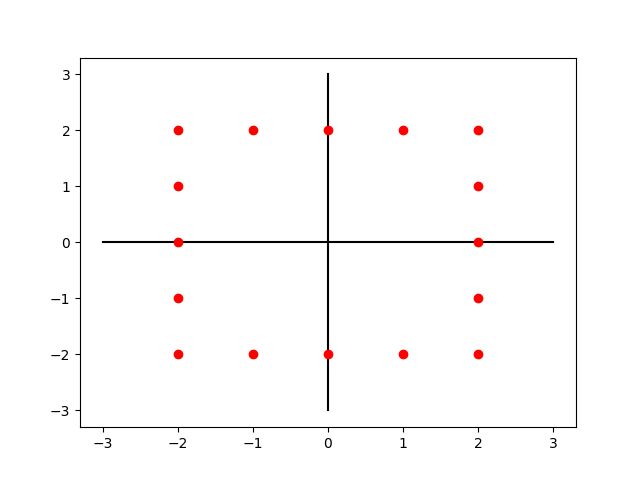
\includegraphics[width=0.7\textwidth]{plot.png}
    \caption{The plot of $[2,0]$.}
\end{figure}
\FloatBarrier

\section{}


\end{document}